\chapter{Symmetry in \pCf}	
\epigraph{Tyger! Tyger! Burning bright, \\
		In the forests of the night. \\
		What immortal hand or eye,\\
		Could frame thy fearful symmetry?}{William Blake, \emph{The Tyger}} 
Dynamical systems in physics often display symmetry. The electron wavefunction in the ground state of hydrogen, or the gravitational motion of a planet around a star, for instance, display very high degrees of spatial symmetry.  Understanding the symmetries of a system can be incredibly useful to an investigator, since they hint at conserved physical quantities (through Noether's Theorem), and can greatly reduce the complexity of the system in various ways. Before I begin the discussion of the symmetries of \pCf, I will first define what `symmetry' means in this thesis. A system is said to be {\bf equivariant} under a symmetry transformation of the dynamical system if the transformation commutes with the time evolution of the system - that is, for a symmetry transformation $S$ and a dynamical system $\dot{x} = f(x)$, 
\begin{equation}
S \dot{x} = Sf(x) = f(Sx).
\end{equation}

The symmetry relations of \pCf\ are discussed extensively in\rf{GIBSON2009}, which I will present here for the sake of flow\footnote{haha}. 
\section{Unbounded Navier-Stokes}

If we do not impose boundary conditions on the Navier-Stokes equations on an infinite domain, the system will be equivariant under continuous rotational and translational symmetry, as well as the discrete {\bf pointwise inversion} symmetry$\sigma_{xz}$, which has the following action on the system:

\begin{equation}\label{eq:pointwiseinversion}
\sigma_{xz}\Vector{u}\paren{\Vector{x}} = -\Vector{u}\paren{-\Vector{x}}
\end{equation}

While the rotation or translation transformation can be easily conceptualized, the pointwise inversion can provide some difficulty. The easiest way of visualizing the transformation is to view it in a 2D domain instead of in the full 3D, as shown in \figureref{fig:pointwiseinversion}. The proof of the equivariance of Navier-Stokes under these transformations can be found in\rf{Gusyatnikova1989}.

\begin{figure}[h]
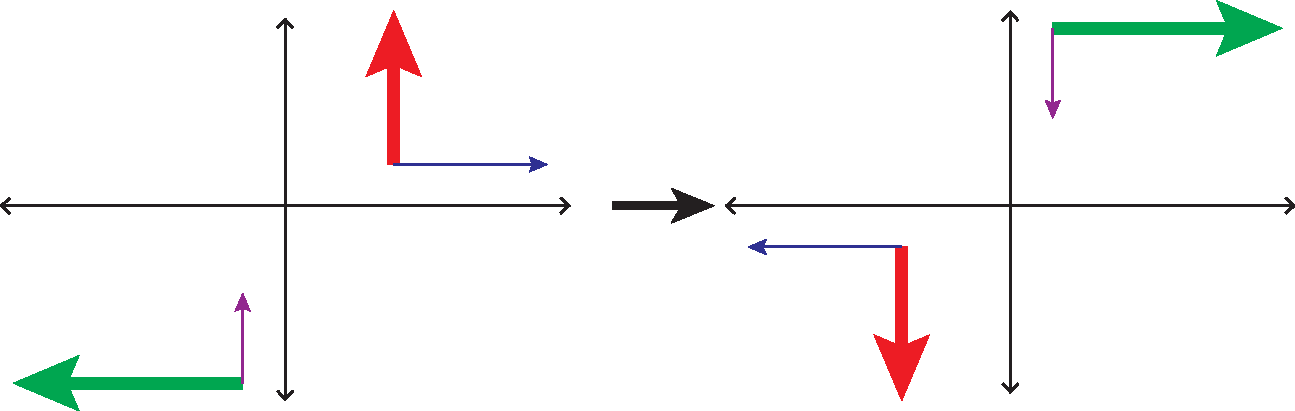
\includegraphics[width=\textwidth]{pointwiseinversion}
\caption{A 2D pointwise inversion operation on two sets of vectors according to \refeq{eq:pointwiseinversion}.}\label{fig:pointwiseinversion}

\end{figure}


\section{Plane Couette Flow}

If the domain is limited to $\mathbb{R}^2 \times [-1,1]$ with the boundary conditions of \pCf, we lose some of the equivariant transformations of the full, unrestricted problem, leaving us with two basic discrete symmetries: a rotation by $\pi$ about the $z$ axis (denoted $\sigma_x$) and a reflection about the $z$ axis (denoted $\sigma_z$)\footnote{The motivation for these subscripts will become apparent shortly}, together form a discrete symmetry group $D = D_1 \times D_1 = \{e, \sigma_x,\sigma_z,\sigma_{xz}\}$ of order 4, where

\begin{align}\label{eq:discretesymm}
\sigma_x [u,v,w](x,y,z) &= [-u,-v,w](-x,-y,z)\\
\sigma_z [u,v,w](x,y,z) &= [u,v,-w](x,y,-z)\\
\sigma_{xz} [u,v,w](x,y,z) &= [-u,-v,-w](-x,-y,-z)
\end{align}

The continuous symmetries are the two parameter steamwise-spanwise translations, which, when provided periodic boundary conditions, form a continuous $SO(2)\times SO(2)$ symmetry group 
\begin{equation}\label{eq:contsymm}
\tau(l_x,l_z)[u,v,w](x,y,z) = [u,v,w](x+l_x,y,z+l_z).
\end{equation}

The group $\Gamma$ of equivariant solutions is then any combination of these symmetry operations, given by $\Gamma = SO(2)_x \ltimes D_{1,x} \times SO(2)_z \ltimes D_{1,z}$\footnote{$\ltimes$ is the semidirect product}. For a solution $\Vector{u}$ of \pCf, the group $s$ of symmetries that satisfies $s\Vector{u} = \Vector{u}$ is called the isotropy subgroup of $\Vector{u}$ and is said to fix $\Vector{u}$. Examples of such groups include the identity group $\{e\}$, which is typically the isotropy subgroup of turbulent solutions. Before I discuss the isotropy subgroup considered for this thesis, however, I will first highlight the useful properties of some particular symmetry subgroups to motivate the eventual choice of isotropy subgroup. 

\section{Properties of $\Gamma$}

It should be evident that since \pCf\ is equivariant under the continuous translations given in \eqref{eq:contsymm}, trajectories can be traveling wave equilibria or relative periodic orbits: that is, if one moves into a different reference frame, the trajectory is a regular equilibrium or periodic orbit. However, an initial condition that is fixed by $\sigma_z$ cannot be translated in the spanwise direction without losing $\sigma_z$ symmetry (except for the trivial case where $\pder{1}{\Vector{u}_z}{z} = 0$). Similarly, an initial condition that is fixed by $\sigma_x$ cannot be translated in the streamwise direction without losing $\sigma_x$ symmetry (and an initial condition that is fixed by $\sigma_{xz}$ symmetry cannot be translated at all without losing $\sigma_{xz}$ symmetry). Since these symmetries are also invariant\footnote{That is, if the symmetry is satisfied at time $t = t_0$, it must be satisfied for all times.}, a trajectory with one of the discrete symmetries cannot be a traveling wave in the direction corresponding to its subscript. \\

The presence of the periodic boundary conditions also implies that all solutions are fixed by the full-period translation $\tau(L_x,0)$ and $\tau(0,L_z)$. However, solutions can also be fixed by any rational translation of the form $\tau(a L_x,b L_z)$, where $a,b \in \mathbb{Q}$, or by the continuous translations. If we fix $\Vector{u}$ by a continuous translation, we force it to have a zero derivative along that axis\footnote{That is, if we fix $\Vector{u}$ by $\tau{l_x,0}$ for any real $l_x$, then $\pder{1}{\Vector{u}}{x} = 0$, and similarly for $z$.}, and such solutions tend to be uninteresting as they are equivalent to low-dimensional problems. If $\Vector{u}$ is fixed instead by rational translations, the periodic cell is tiled with repeating subcells , as in \refFig{fig:rationalTranslation}. This implies that we can restrict ourselves to full box length translations, which are in any case required by the periodic boundary conditions.
 \begin{figure}[h]
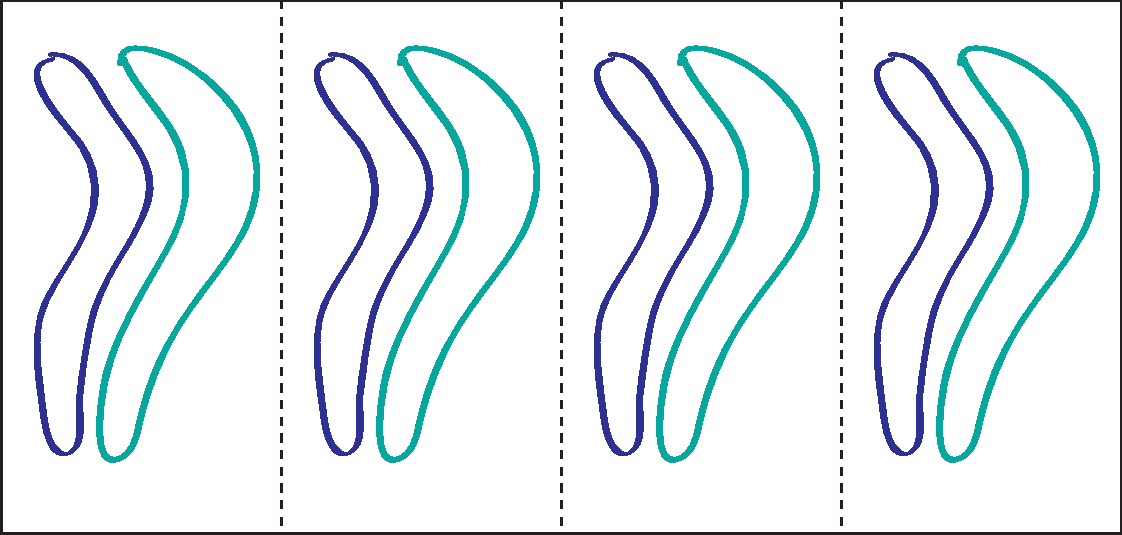
\includegraphics[width=\textwidth]{SubCell}
\caption{If the flow state is fixed by $\tau(\dfrac{1}{4}L_x,0)$, then the cell will have four repeating streamwise subcells, and it becomes more efficient to solely consider the subcell.}\label{fig:rationalTranslation}

\end{figure}

Finally, we can reduce the number of unique subgroups of $\Gamma$ by considering its {\bf conjugacy groups}. A group $N$ and $M$ are considered conjugate if for some $s \in \Gamma$, $N = s^{-1}Ms$ - that is, $N$ and $M$ are related by a coordinate transformation. This allows us to consider only one group out of a set of mutually conjugate groups (known as a conjugacy class), since any other group in the class is simply related by the application of a symmetry transformation. This becomes especially important when considering $O(2) =  SO(2) \ltimes D_{1}$, since it is not an abelian group as reflections and translations about the same axis are noncommutative (\refFig{fig:notabelian}). However, we can still recover a psuedo-commutative relation by considering \figureref{fig:abelian}. We can see that $\sigma_z\tau_z$ results in the object moving by $l_z$ to the right, and the being mirrored across the $z$ axis, at which point it is mirrored and $l_z$ to the left of the origin. We can achieve the same effect by mirroring the object and moving it to the left - that is, applying the operation $\tau_z^{-1}\sigma_z$, leading us to conclude that $\sigma\tau = \tau^{-1}\sigma$. We can rewrite this as $\sigma\tau^2 = \tau^{-1}\sigma\tau$, so
\begin{equation}
\sigma_x\tau(l_x,0) = \tau^{-1}(l_x/2,0)\sigma_x\tau(l_x/2,0),
\end{equation}

\begin{figure}[t!]
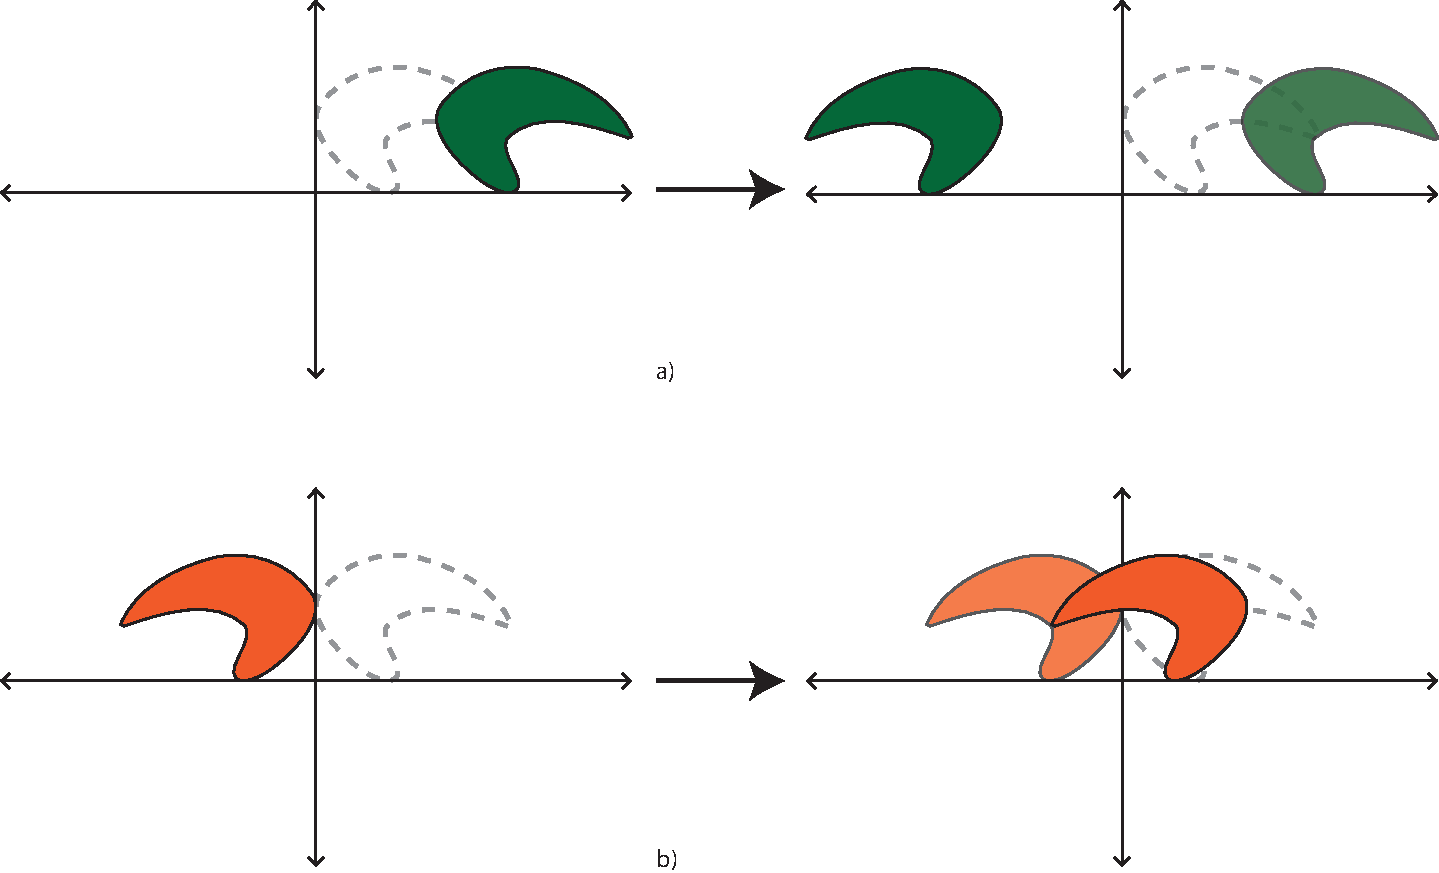
\includegraphics[width=\textwidth]{shiftReflectNotCommuting}
\caption{A simple demonstration that shifts and reflects do not commute in general. a) shows an object with a dashed outline that is translated to the right, and then reflected across the vertical, while b) shows the same object reflected before it is translated to the right. Notice that the final positions of the object are not the same.}\label{fig:notabelian}
\end{figure}

\begin{figure}[t!]
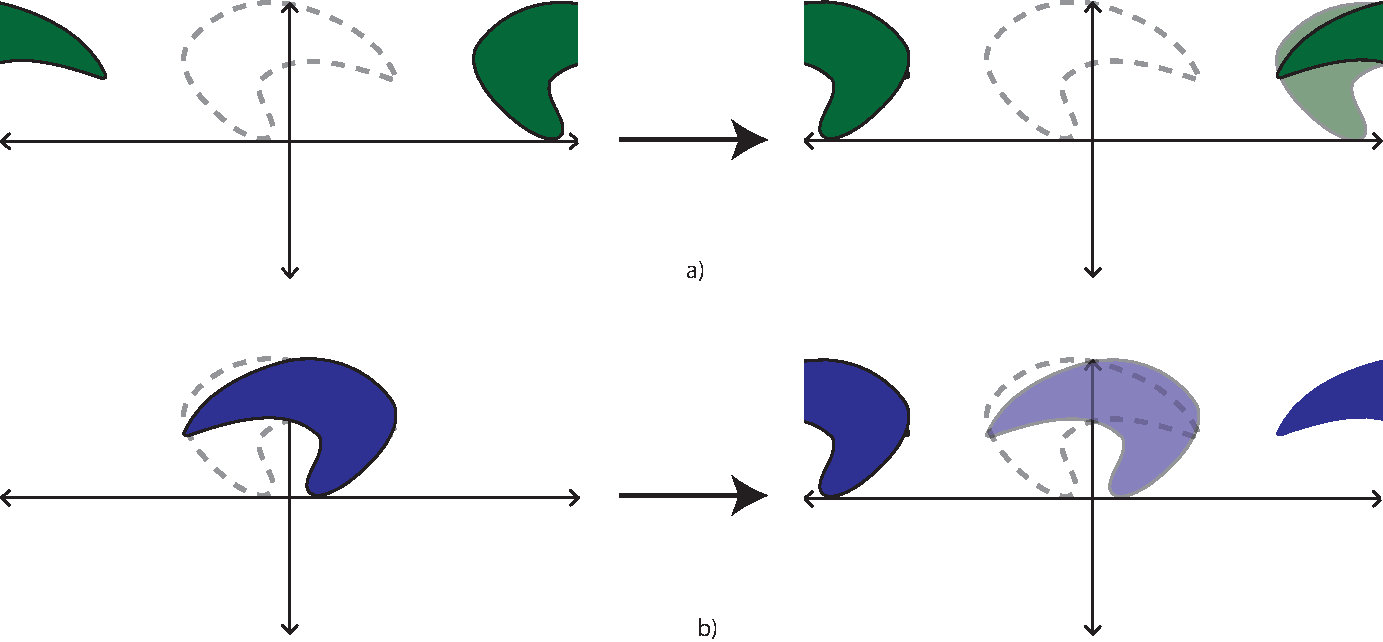
\includegraphics[width=\textwidth]{shiftReflectCommuting}
\caption{When periodic boundary conditions are imposed and translations are fixed to half-period lengths, shifts and reflects commute. a) shows an object that is shifted and then reflected across the vertical, while b) shows the same object reflected across the vertical and then shifted. Notice that the final positions are the same, even if the indermediaries are not.}\label{fig:abelian}
\end{figure}
which implies that $\sigma_x$ and $\sigma_x\tau_x$ are part of the same conjugacy class - so if a isotropy group contains $\sigma_x\tau_x$, there is a simpler version of that group which contains $\sigma_x$ instead. Note that if $l_x = L_x$, then we have $\sigma_x = \tau_x^{-1}\sigma_X\tau_x$, so reflection and translations commute for any half-integer cell shifts. In this thesis, I will work with either half-cell or or null shifts. The group of half cell shifts is denoted $C_2$, so the group 
\begin{align}
G &= D_{1,x} \times C_{2,x} \times D_{1,z} \times C_{2,z} \subset \Gamma
\end{align} 

is an abelian group of order 16, containing both the isotropy groups of half-cell and null shifts.

\section{Symmetry Groups of this Thesis}

We can categorize the conjugacy classes of $G$ by their order - in this thesis, we will work with order 2 and 4 classes. There are 15 subgrups of order-2 (since there are 15 non-identity elements in $G$), 35 subgroups of order 4 ($(15\cdot14) /(3\cdot2)$), 15 subgroups of order 8 and 1 subgroup of order 16, giving 67 subgroups of $G$. Luckily, the existence of conjugacy classes allow us to greatly simplify the number of distinct groups we need to consider. For order-2 subgroups, conjugacy between $\sigma_x$ and $\sigma_x\tau_x$ and $\sigma_z\tau_z$ allows us to simplify down to just 8 distinct groups, which are generated by $\sigma_x,\sigma_z,\sigma_{xz},\sigma_x\tau_z,\sigma_z\tau_x,\tau_x,\tau_z,\tau_{xz}$. Recalling the behavior of these symmetries, we can see that only $\sigma_{xy}$ generates a group without travelling waves, $\sigma_z$ and $\sigma_z\tau_x$ generate groups that allow travelling waves in the $x$ direction, $\sigma_x\tau_z$ and $\sigma_x\tau_z$ generate groups that allow travelling waves in the $z$ direction, and the pure translations allow travelling waves in any (in-plane) direction. \\

  
